\documentclass[12pt,a4paper]{article}
\usepackage[utf8]{inputenc} % sempre salve seus arquivos como UTF8
\usepackage[T1]{fontenc}
\usepackage[english]{babel}

\usepackage[left=2.5cm,right=2cm,top=2cm,bottom=2.5cm]{geometry}
\usepackage{amsmath}
\usepackage{amsthm}
\usepackage{amsfonts}

\usepackage{graphicx}
\usepackage{algorithm}
\usepackage{color}
\usepackage[noend]{algpseudocode}
\usepackage{mathtools}
\usepackage{subfig}
\usepackage{diagbox}

% load times font
\usepackage{mathptmx}
\usepackage[scaled=.90]{helvet}
\usepackage{courier}

% comandos
\newcommand{\mdc}[1]{\mathrm{mdc}(#1)}

\DeclarePairedDelimiter\ceil{\lceil}{\rceil}
\DeclarePairedDelimiter\floor{\lfloor}{\rfloor}

% Foot without marker
\newcommand\blfootnote[1]{%
	\begingroup
	\renewcommand\thefootnote{}\footnote{#1}%
	\addtocounter{footnote}{-1}%
	\endgroup
}

\title{MO446 -- Introduction to Computer Vision  \\ Project 3}
\author{Breno Leite  \\ Guilherme Leite}
\date{05/10/2017}

\begin{document}

\maketitle
\blfootnote{\textit{\textbf{Important note:} The borders seen in the figures are not part of the image, they are figurative information about the starting and ending points of the image. Moreover, all the image scales in this report were changed in order to make the text more readable.}} \\

%% ---------------- Starts here --------------------------------

\textbf{\LARGE Question 2 - Input Data} \\

The input data used in this project was obtained with a cellphone camera,  recording the magic cube from Figure \ref{fig:magicCube}. Two videos were taken, the first one (\textbf{p3-1-0}) shows a translation movement (affine transformation) of the magic cube in a "blank" background and was used in the experiments of Question 4 - Feature Tracking. The second (\textbf{p3-1-1}) shows the magic cubic performing a rotation movement and it was used in Question 5 - Structure from Motion experiments. \\

\begin{figure}[!h]
	\centering
	{
		\setlength{\fboxsep}{1pt}
		\setlength{\fboxrule}{1pt}
		\fbox{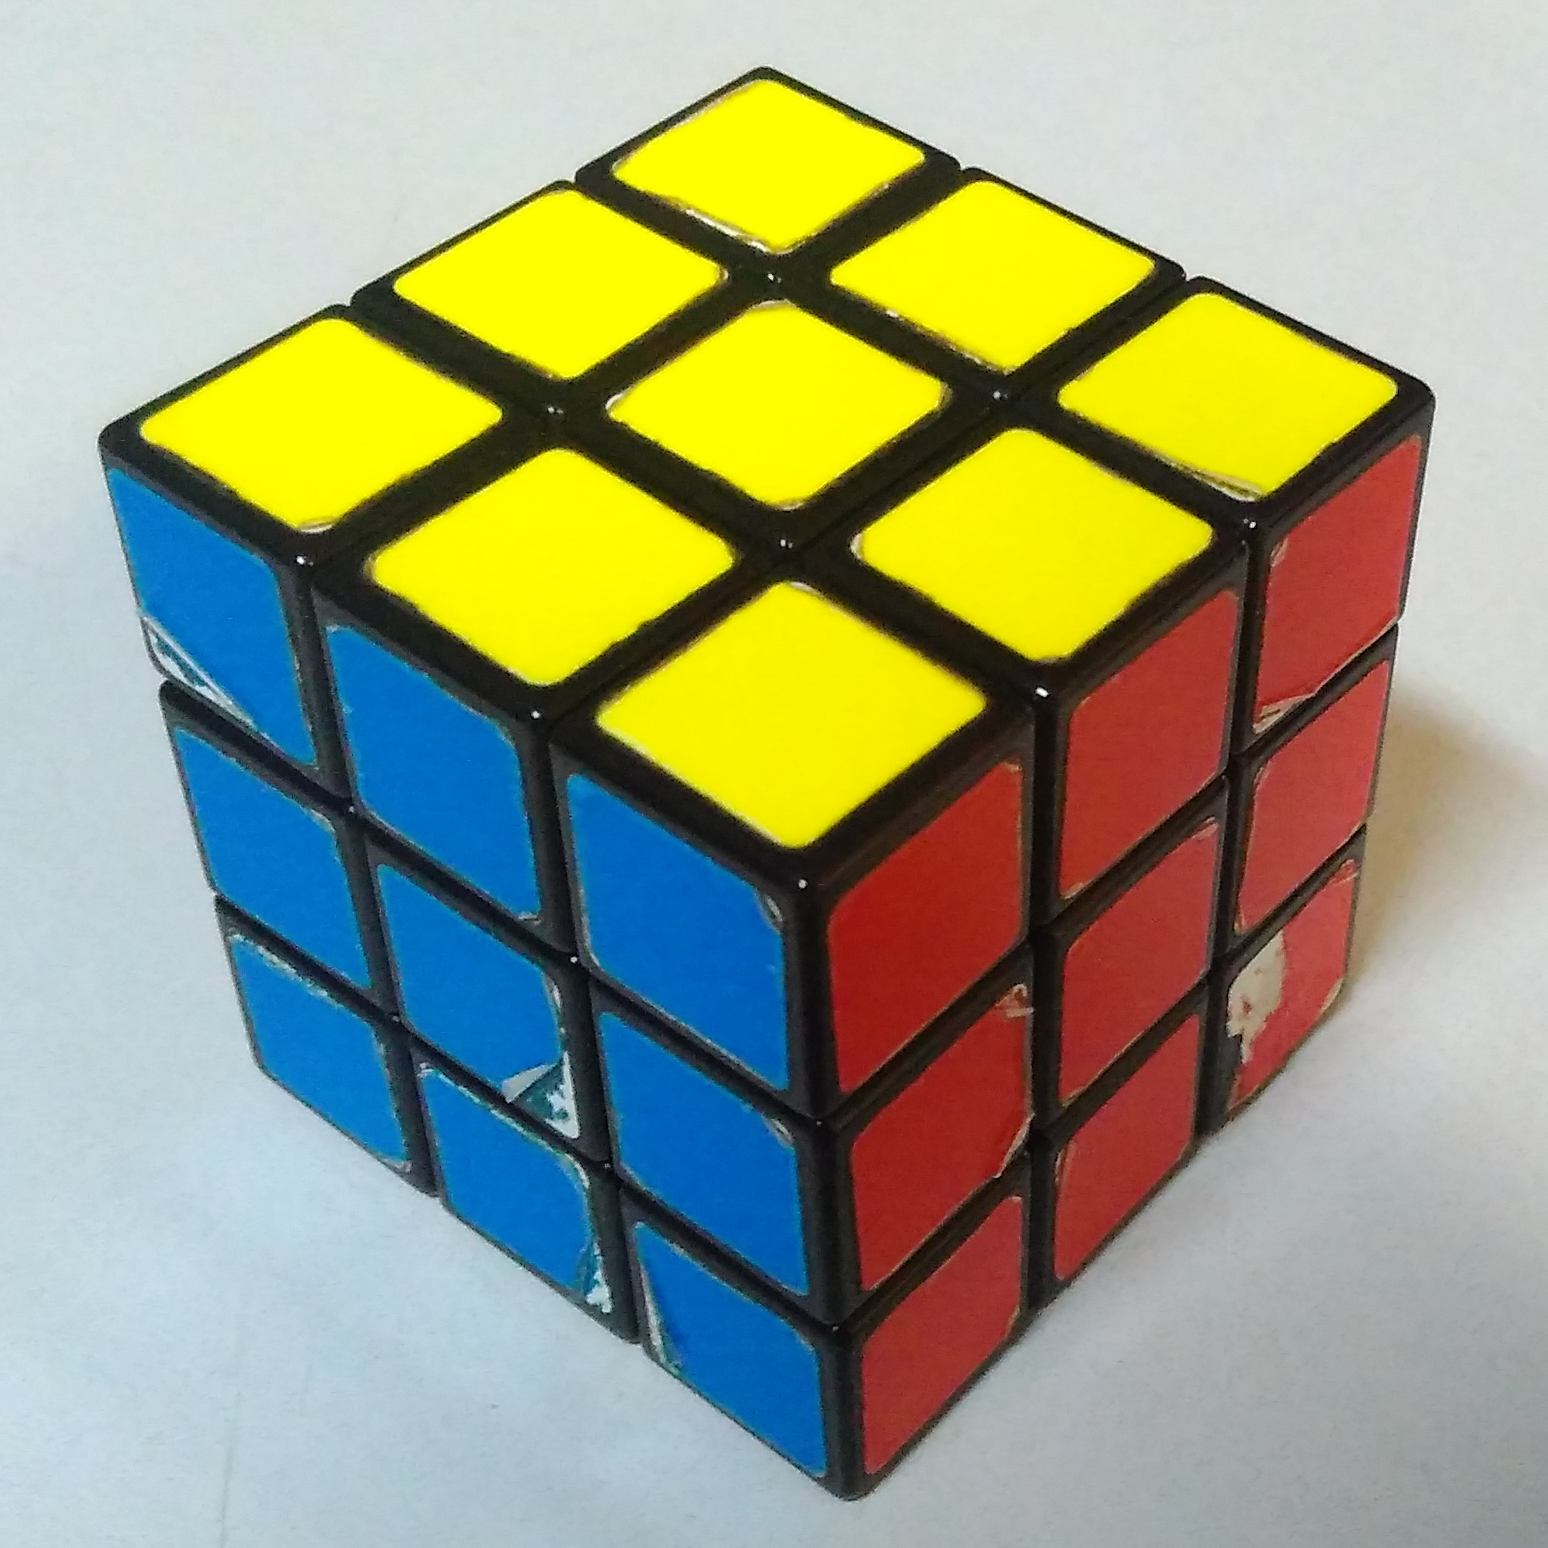
\includegraphics[scale=0.1]{report/magicCube}}
	}
	\caption{Magic cube used in the video recordings.}
	\label{fig:magicCube}
\end{figure}

\textbf{\LARGE Question 3 - Keypoint Selection} \\

The Harris and SIFT keypoint detector (KP detector) were explored in this project. The most noticeable difference between them is the amount of keypoints extracted, the SIFT algorithm extracts more keypoints than Harris, see Figure \ref{fig:keypointSelection}. However the SIFT is more time expensive, in this experiment it took 0.0736 seconds to extract the keypoints, while the Harris took just 0.0067 seconds. \\

\begin{figure}[!h]
	\centering
	\subfloat[Using Harris detector (\textbf{p3-3-0}).]{
		{
			\setlength{\fboxsep}{1pt}
			\setlength{\fboxrule}{1pt}
			\fbox{\includegraphics[scale=0.3]{output/p3-3-0}}
		}
		\label{fig:keypointSelectionHarris}
	}
	\quad
	\subfloat[Using SIFT detector (\textbf{p3-3-1}).]{
		{
			\setlength{\fboxsep}{1pt}
			\setlength{\fboxrule}{1pt}
			\fbox{\includegraphics[scale=0.3]{output/p3-3-1}}
		}
		\label{fig:keypointSelectionSift}
	}
	\caption{Difference between keypoint detection methods.}
	\label{fig:keypointSelection}
\end{figure}

Considering that the keypoints will be used later on the object flow, it is vital to obtain points regarding only the magic cube in this step. Using Harris detector many corners of the magic cube were selected and as seen in Figure \ref{fig:keypointSelectionHarris} not a single keypoint outside the magic cube boundaries was selected. The same does not hold for SIFT, Figure \ref{fig:keypointSelectionSift}, since it's based on gradients a few points outside the magic cube boundaries were selected. Figure \ref{fig:keypointSelectionSiftPoints} highlights in yellow  these selected  keypoints, the main reasons for that are the shadows in the image and other objects that appears in the scene like the thread.\\
	
\begin{figure}[!h]
	\centering
	{
		\setlength{\fboxsep}{1pt}
		\setlength{\fboxrule}{1pt}
		\fbox{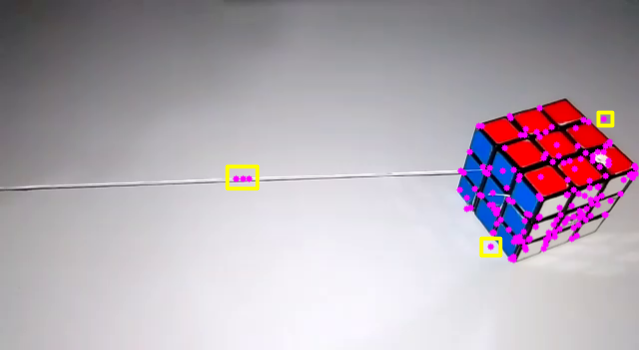
\includegraphics[scale=0.6]{report/out_points}}
	}
	\caption{SIFT highlighted keypoints.}
	\label{fig:keypointSelectionSiftPoints}
\end{figure}

	

%%---------------------------------------------------------------------

\newpage

\textbf{\LARGE Question 4 - Feature Tracking} \\

In this section the results obtained in the optical flow will be shown. The video \textbf{p3-1-0} was used, which contains basically a translation movement. Two different videos were created in this section (\textbf{p3-4-0} and \textbf{p3-4-1}), the first video shows the results using  Harris keypoint detector. In other hand, the second video shows results of optical flow using SIFT detector. Both videos are showing the results of our implementation (Left image, green color) and the OpenCV implementation (Righ image, pink color). \\

In \textbf{Question 3} it was shown that SIFT usually finds more keypoints than  Harris corner detection, however, it is more expensive. A time comparison for the optical flow is shown in Table \ref{table:flowTime}. \\


\begin{table}[!h]
	\centering
	\begin{tabular}{|c|c|c|}
		\hline
		& \multicolumn{2}{c|}{Time (seconds)} \\ \hline
		\backslashbox{\textbf{Implementation}}{\textbf{KP Detector}}      & Harris            & SIFT            \\ \hline
		Ours   & 3.79              & 26.20           \\ \hline
		OpenCV & 0.57              & 0.86            \\ \hline
	\end{tabular}
	\caption{Comparison between our implementation and OpenCV's for optical flow.}
	\label{table:flowTime}
\end{table}

As seen the SIFT is really more expensive, the reason for that is not only SIFT is, by its own, less time efficient than Harris but the large number of keypoints found by SIFT increases the cost of computing the optical flow. Because of the better performance, and also for easiness on the results visualization the Harris implementation was used in some of the experiments in this section. \\

Picking a good neighbourhood size is essential for the optical flow algorithm, the Figure \ref{fig:keypointSelection} shows some comparisons between different sizes of neighbourhoods. The images were taken from the first, middle, and last frame in the video (left to right). \\

\begin{figure}[!h]
	\centering
	{
		{
			\setlength{\fboxsep}{1pt}
			\setlength{\fboxrule}{1pt}
			\fbox{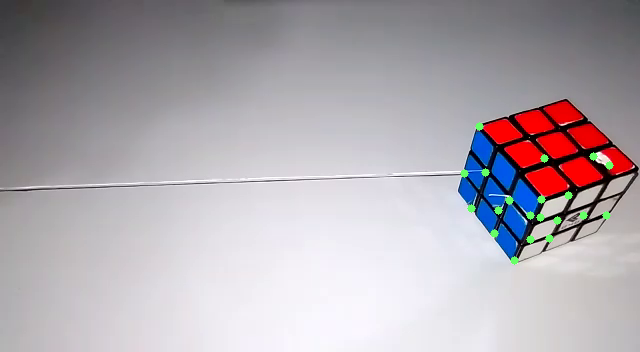
\includegraphics[scale=0.2]{report/7s}}
		}
	}
	\enskip
	{
		{
			\setlength{\fboxsep}{1pt}
			\setlength{\fboxrule}{1pt}
			\fbox{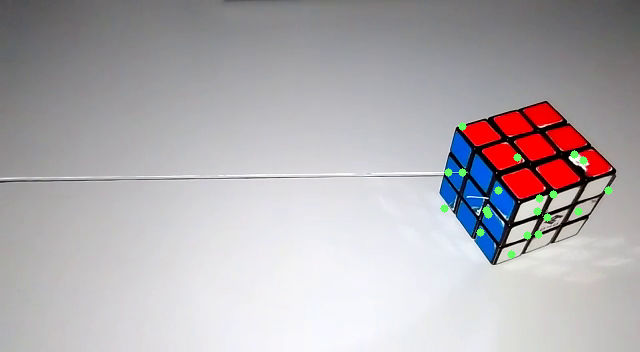
\includegraphics[scale=0.2]{report/7m}}
		}	
	}
	\enskip
	{
		{
			\setlength{\fboxsep}{1pt}
			\setlength{\fboxrule}{1pt}
			\fbox{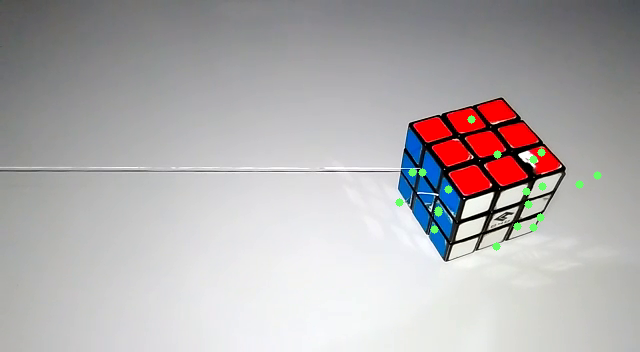
\includegraphics[scale=0.2]{report/7l}}
		}	
	}
	
	%---------------
	{
		{
			\setlength{\fboxsep}{1pt}
			\setlength{\fboxrule}{1pt}
			\fbox{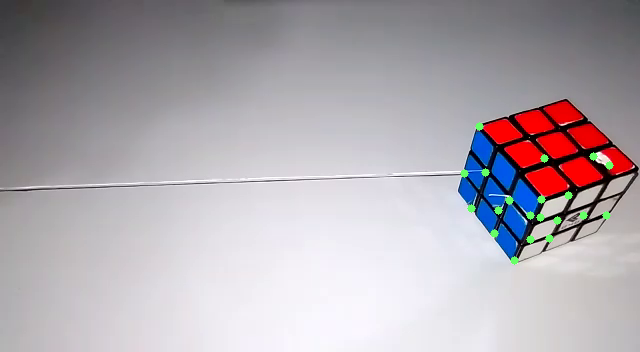
\includegraphics[scale=0.2]{report/15s}}
		}
	}
	\enskip
	{
		{
			\setlength{\fboxsep}{1pt}
			\setlength{\fboxrule}{1pt}
			\fbox{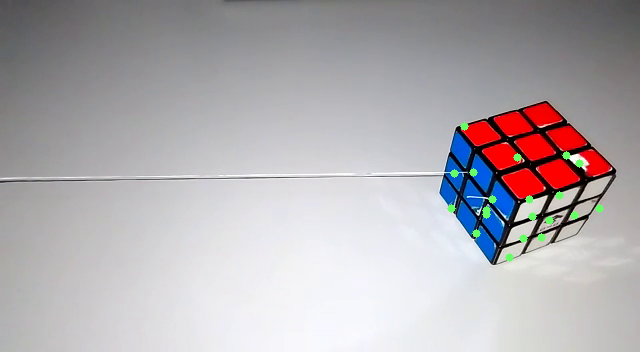
\includegraphics[scale=0.2]{report/15m}}
		}	
	}
	\enskip
	{
		{
			\setlength{\fboxsep}{1pt}
			\setlength{\fboxrule}{1pt}
			\fbox{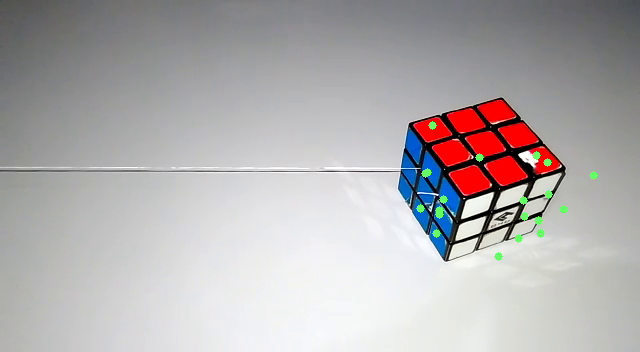
\includegraphics[scale=0.2]{report/15l}}
		}	
	}
		
	%---------------
	{
		{
			\setlength{\fboxsep}{1pt}
			\setlength{\fboxrule}{1pt}
			\fbox{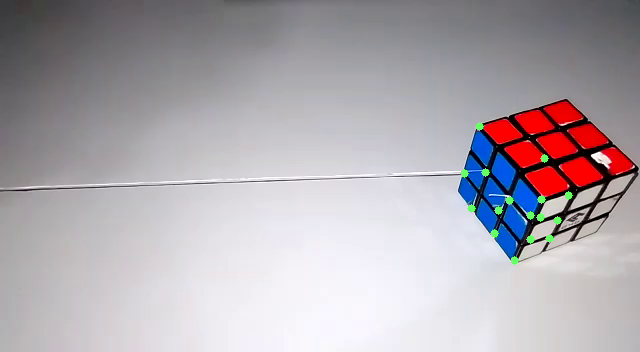
\includegraphics[scale=0.2]{report/30s}}
		}
	}
	\enskip
	{
		{
			\setlength{\fboxsep}{1pt}
			\setlength{\fboxrule}{1pt}
			\fbox{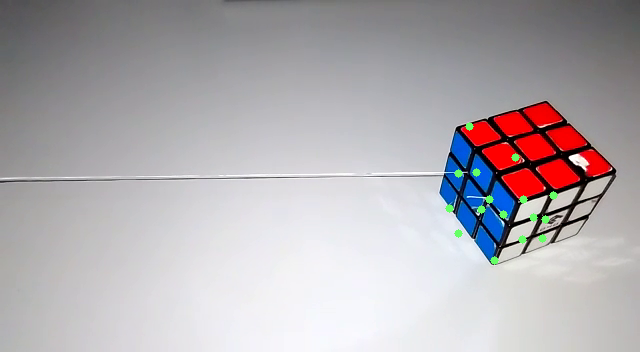
\includegraphics[scale=0.2]{report/30m}}
		}	
	}
	\enskip
	{
		{
			\setlength{\fboxsep}{1pt}
			\setlength{\fboxrule}{1pt}
			\fbox{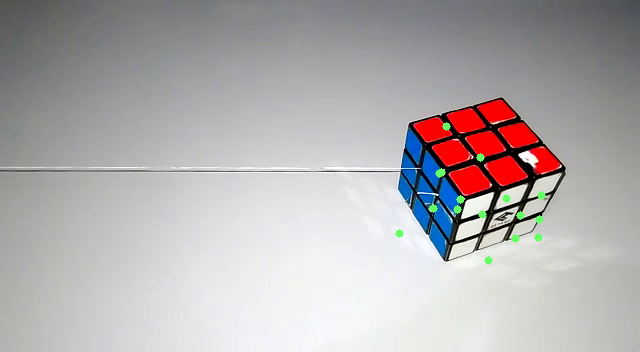
\includegraphics[scale=0.2]{report/30l}}
		}	
	}
	
	\caption{Three different frames from the video using $7x7$, $15x15$, and $30x30$ neighborhood, respectively in each row.}
	\label{fig:keypointSelection}
\end{figure}

The results shows that the keypoints normally falls behind from the actual movement of the object, the first row (representing the $7x7$ neighborhood) is the most affected by this problem. On the other hand, the last row (representing $30x30$) is the most accurate on the points. However, the number of keypoints is really smaller than the others. \\

The reason for this is the border filtering, as the neighborhood increases more keypoints needs to be removed from the border in order to maintain the algorithm boundaries. This filtering process removes some keypoints, as seen in the last image from the first column (which represents the first frame of the video). Note that for the $7x7$ and $15x15$ neighborhood the image is identical. \\

The $15x15$ neighborhood has shown the best results, it does not lack the number of keypoints as the $30x30$ neighborhood and it also does not suffer as much as the $7x7$ neighborhood from falling behind the object. Because of this the $15x15$ neighborhood has been selected to generate the video. The Figure \ref{fig:flowVideo} shows the motion flow on the last frame from the video using Harris keypoint detector. \\

\begin{figure}[!h]
	\centering
	\subfloat[Our implementation.]{
		{
			\setlength{\fboxsep}{1pt}
			\setlength{\fboxrule}{1pt}
			\fbox{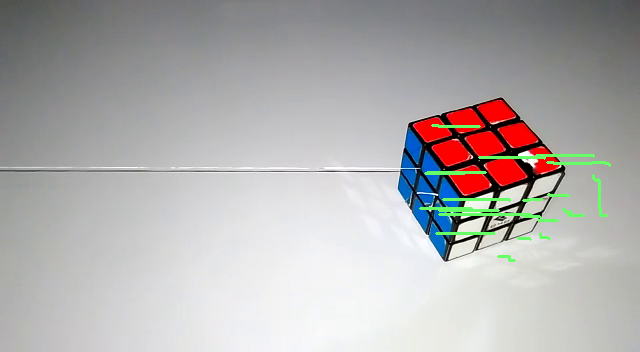
\includegraphics[scale=0.3]{report/videoFlow}}
		}
		\label{fig:videoFlowOur}
	}`
	\enskip
	\subfloat[OpenCV implementation.]{
		{
			\setlength{\fboxsep}{1pt}
			\setlength{\fboxrule}{1pt}
			\fbox{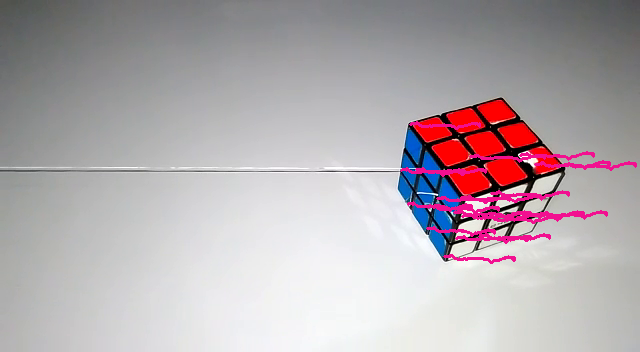
\includegraphics[scale=0.3]{report/videoFlow_OpenCV}}
		}
		\label{fig:videoFlowCV}
	}
	\caption{Last frame from video showing results on optical flows using Harris Keypoint Detector (\textbf{p3-4-0}).}
	\label{fig:flowVideo}
\end{figure}

The Figure \ref{fig:videoFlowOur} shows the optical flow of the object, however, it is noticeable that the keypoints are falling behind the object. This effect could be optimized using other techniques such as pyramids or even recomputing the keypoints after a certain amount of frames. None of this approaches were implemented in this work. As seen the OpenCV implementation tracks the keypoints with more precision than our implementation, see Figure \ref{fig:videoFlowCV}.  \\


%%---------------------------------------------------------------------

\newpage

\textbf{\LARGE Question 5 - Structure from Motion} \\

In this section we used the OpenCV implementation of optical flow, the reason is that it is more consistent which enables better reconstruction performance. We tested our implementation, however, the falling behind keypoints on the video used in (\textbf{p3-1-1}) did not perform well. Therefore, the SIFT keypoint detector was used throughout the experiments. As shown before, it detects more keypoints which gives a better reconstruction of the 3D world. \\

We checked the number of points necessary to the reconstruction by a process of trial and error, the number of keypoints given by Harris keypoint detector was not sufficient to make a good 3D reconstruction. We have also satisfied the equation proposed by Morita et. al. and  $2F > P$, in which $F$ is the number of frames from the video, and $P$ is the number of ``good keypoints'' \blfootnote{http://cs.brown.edu/courses/cs143/2011/proj5/Morita\_Kanade\_PAMI\_1997.pdf}. ``Good keypoints'' are those which never goes out of the camera's view. \\

The Figure \ref{fig:3dframe} shows the first frame of the image, which is where the SIFT keypoint detector is used. The motion from this points will be responsible for the 3D structure reconstructed.

\begin{figure}[!h]
	\centering
	{
		\setlength{\fboxsep}{1pt}
		\setlength{\fboxrule}{1pt}
		\fbox{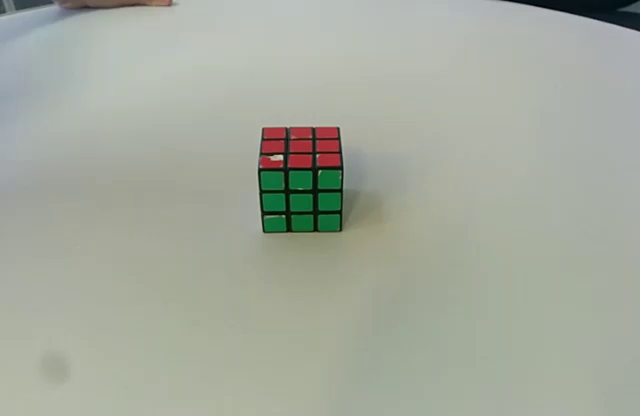
\includegraphics[scale=0.4]{report/3dframe}}
	}
	\caption{First frame of the video.}
	\label{fig:3dframe}
\end{figure}

Using the keypoints selected the structure from motion model create the cloud of points represented in  the Figure \ref{fig:3dpoints}.

\begin{figure}[!h]
	\centering
	{
		{
			\setlength{\fboxsep}{1pt}
			\setlength{\fboxrule}{1pt}
			\fbox{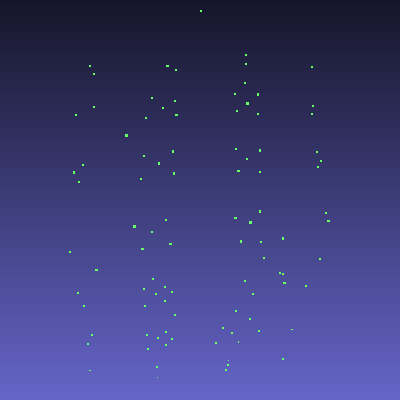
\includegraphics[scale=0.3]{report/3d_points1}}
		}
		\label{fig:3dpoints1}
	}
	\enskip
	{
		{
			\setlength{\fboxsep}{1pt}
			\setlength{\fboxrule}{1pt}
			\fbox{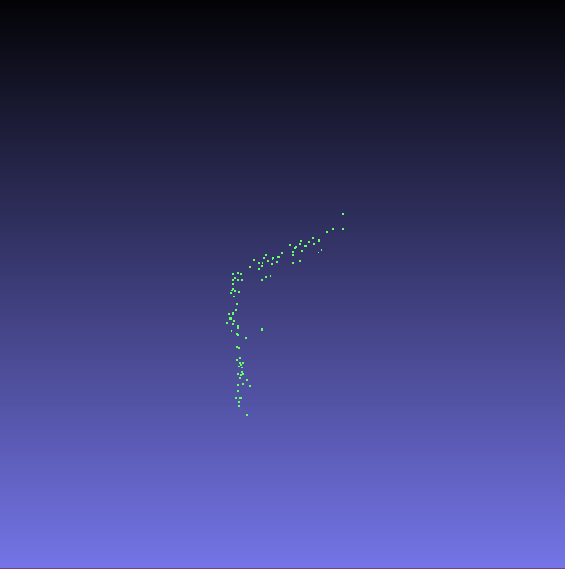
\includegraphics[scale=0.3]{report/3d_points2}}
		}
		\label{fig:3dpoints2}
	}
	\enskip
	{
		{
			\setlength{\fboxsep}{1pt}
			\setlength{\fboxrule}{1pt}
			\fbox{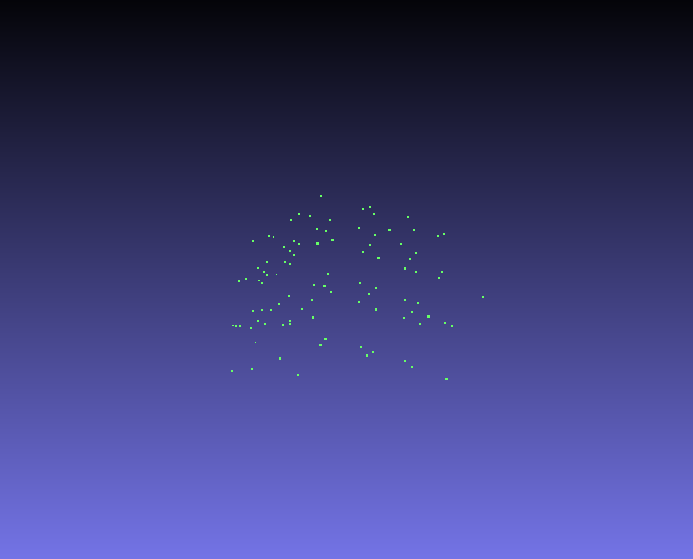
\includegraphics[scale=0.3]{report/3d_points3}}
		}
		\label{fig:3dpoints3}
	}
	\caption{Different angles from cloud of points taken from \textbf{p3-5-0}.}
	\label{fig:3dpoints}
\end{figure}

As seen in the cloud of points, both sides of the cubic was reconstructed into the 3D world. Some adjustments were made in the code for better visualization, like removing some outliers points which were too distant from the object reconstructed. The camera's position/trajectory was also reconstructed from motion, the Figure \ref{fig:3dcamera} shows the cloud of points representing the camera's trajectory.

\begin{figure}[!h]
	\centering
	{
		\setlength{\fboxsep}{1pt}
		\setlength{\fboxrule}{1pt}
		\fbox{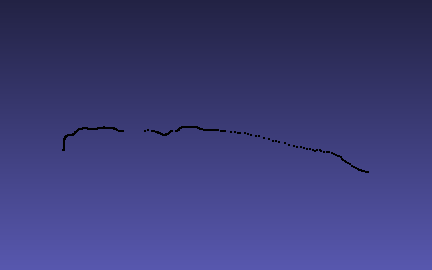
\includegraphics[scale=0.4]{report/3dcamera}}
	}
	\caption{Camera's trajectory reconstructed from the motion.}
	\label{fig:3dcamera}
\end{figure}

This positions were computed using the cross product on the transformation matrix ($M$), where the cross were taken using $M_1 \ cross \ M_{f+1}, M_2 \ cross \ M_{f+2}, \dotso, M_{f-1} \ cross \ M_{2f}$, in which $M_x$ is the $xth$ row of the $M$ matrix. The cross product was used to find a perpendicular vector from the $X$ and $Y$ coordinates from the transformation matrix $M$. In this way the camera's trajectory was reconstructed, and as seen the camera movement follows the rotation of the object. This happens because there is not enough information to check if the camera or the object is moving. \\



 
\end{document}
